\documentclass[a4paper]{article}

\usepackage{graphicx}
\usepackage{minted}
\usepackage{xspace}
\usepackage{verbatim}

\newcommand{\starcraft}{StarCraft\xspace}

\title{Java Behaviour Trees, User Guide}
\author{Ricardo Juan Palma Dur\'an}

\begin{document}
\maketitle
\vspace{-0.5cm}

\tableofcontents
\clearpage

\section{Introduction}

Java Behaviour Trees (JBT) is a Java framework for building and running behaviour trees (BTs). In the past few years, BTs have been widely accepted as a tool for defining the behaviour of video games characters. However, to the best of our knowledge, there is no free-software Java implementation of such technology. With JBT we intend to provide a solid framework to build and run BTs in Java.

JBT has two main parts. On the one hand, there is the JBT Core (it is the Eclipse SDK project under the "./JBTCore" directory of the repository), which implements all the classes needed to create and run BTs. JBT Core basically lets the user create BTs in pure Java and then run them. In order to ease the task of creating BTs, JBT Core includes several tools that automatize the process of creating BTs. In particular, it can create the Java source code of a BT from its description in an XML format. By doing so, the user of this framework basically has to worry only about defining BTs in XML files and implementing the low level actions and conditions that his trees will use, which are domain-dependant (that is, they depend on the game being played). We provide a .jar file with all the JBT Core classes. Of course, in order to get the last version of the JBT Core the repository can be accessed.

On the other hand, there is the JBT Editor (which is composed of two Eclipse SDK projects under the "./JBTEditor" directory of the repository). The JBT Editor is a GUI application that can be used for defining BTs, and then exporting them into XML files in the format that the JBT Core understands. The JBT Editor offers a set of standard nodes\footnote{Note that, when talking about BTs, \textit{node} and \textit{task} are used interchangeably.} for building BTs. It includes nodes such as sequences, parallels, decorators, etc. For low level actions and conditions, the user can provide their conceptual definition through Make Me Play Me (MMPM) domain files (for more information on MMPM, see the Sourceforge page of the project "Darmok 2"). The JBT Editor is an Eclipse RCP application, so you must use Eclipse SDK in order to run it. An alternative to run it is to use the executable files provided for each platform. Of course, if order to get the last version of the JBT Editor the repository can be accessed.

JBT implements a BT model which is mainly based on that of the book "Artificial Intelligence for Games", second edition, by Ian Millington and John Funge. JBT also includes the concept of "guard" and static and dynamic priority lists, which make use of guards. JBT BTs are driven by ticks, which means that, in order for them to have CPU time, they need to be externally ticked. By following this pattern, the user can control how much CPU time the BT consumes.

In this document we explain how JBT can be used to build and run BTs. This process has the following steps:

\begin{itemize}
  \item Defining low level actions and conditions to be used in the trees. These actions and conditions are defined in the MMPM format.
  \item Implementing the low level actions and conditions. The user has to define how the low level actions and conditions work. JBT does not know how these domain-dependent actions and conditions work, so the user has to provide a Java implementation of them.
  \item Creating BTs with the JBT Editor. Here, the user creates BTs that are exported into generic XML files.
  \item Creating the Java declaration of the BTs that were declared in the XML files. This is automatically done by one of JBT's tools.
  \item Running the BTs by using the core classes of JBT. 
\end{itemize}

In the next sections we will describe all of these steps. Also, we will conceptualize them through a real example on a real game, since we will build a tree that is able to control a Terran Marine of the Real Time Strategy Game \starcraft.

\section{JBT, an Overview}

In this section we describe the JBT architecture as well as the main features that BTs have.

\subsection{Model Driven by Ticks}\label{sec:ModelDrivenByTicks}

JBT implements a BT model driven by ticks. A BT must be evaluated through ticks, so every game cycle an external caller \textit{ticks} the tree in order for the tree to update its status. A tick is just a way of giving the tree some CPU time to update their status; in particular, ticks are used to give the nodes of the tree some time to evaluate whether they have finished or not, and consequently make the tree evolve.

The simplest approach to BTs driven by ticks is that of ticking the root node and then letting each node recursively tick its children according to its semantics. However, this is a very inefficient process, since in general the major part of the nodes of the tree are just waiting for their children to finish. Therefore, they should not receive ticks, since unless their children are done they will do nothing useful when receiving the tick. Therefore, in general only very few nodes should be ticked at a game cycle, and as a result JBT implements a model in which there is a list of \textit{tickable} nodes. Only the nodes in the list can be ticked.

\subsection{Model Independent from Execution}\label{sec:ModelIndependentFromExecution}

When running a BT, there should be a clear distinction between the tree that is being run (the model) and how it is actually being run (the execution). For each particular behaviour, we distinguish between the \textit{Model BT} that defines it and how it is being run. The \textit{how} is what the \textit{BT Executor} does. Basically, for every entity in the game that wants to run a behaviour (Model BT), there is a BT Executor. The BT Executor takes the Model BT and processes it (without modifying it), simulating the behaviour that is represented by the Model BT. This choice implies that, apart from the Model BT, there is another type of tree, the \textit{Execution BT}. When an entity wants to execute a behaviour, the BT Executor takes the Model BT and creates an Execution BT to execute the behaviour. The BT Executor along with the Execution BT know how to run the behaviour that the Model BT represents.

\subsection{Architecture}\label{sec:Architecture}

Figure \ref{fig:Overview} shows an overview of the JBT Core architecture. There is a Model BT that represents a particular behaviour. Also, there is a BT Executor for every entity that wants to run the Model BT. Each BT Executor makes use of the Model BT and builds an Execution BT that actually runs the behaviour conceptualized by the Model BT. An external Game AI ticks the BT Executors, in order for them to update the trees that they are running.

\begin{figure}
 \centering
 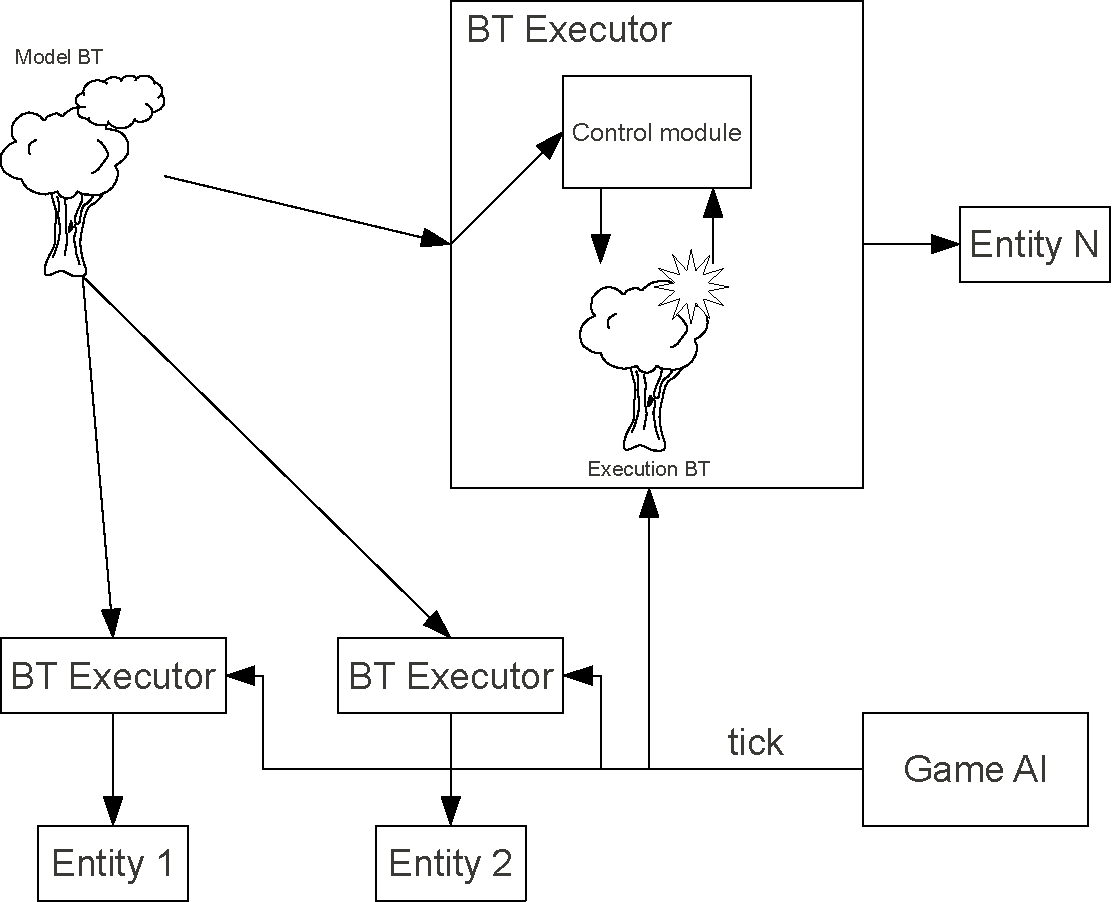
\includegraphics[width=\textwidth]{./Images/Overview.pdf}
 \caption{Overview of the BT architecture}
 \label{fig:Overview}
\end{figure}

The user of the framework does not have to know all the details about how JBT internally works. However, since he has to implement some classes in order to run his own trees, at least he should know the general architecture of JBT.

\subsection{BT Model}\label{sec:BTModel}

Before even starting to explain all the steps required to build and run BTs with JBT, we have to first think about what BT model JBT offers. JBT implements a BT model that is mainly based on that of \cite{Millington09}. Our model also include guards and static and dynamic priority lists, as described in \cite{QueryEnabledBTs}. With this model the user can implement a wide range of behaviours. 

For instance, the tree of figure \ref{fig:SimpleOpenDoor} represents a simple tree that is used by a game character that wants to open a door. First of all, it checks if the door is closed (condition \textit{DoorClosed}). If so, then it tries to open it by executing the action \textit{OpenDoor}.

\begin{figure}
 \centering
 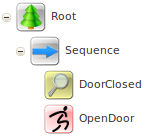
\includegraphics[width=0.3\textwidth]{./Images/SimpleOpenDoor.png}
 \caption{a simple behaviour tree}
 \label{fig:SimpleOpenDoor}
\end{figure}

In the tree of figure \ref{fig:SimpleOpenDoor} we can see four nodes. The node called \textit{Root} is just the root of the tree, and it has no actual meaning apart from it. Then there is a \textit{Sequence} node, which runs in sequence both of its children, the \textit{DoorClosed} condition and the \textit{OpenDoor} action. The Sequence node is a standard node, but both the DoorClosed and the OpenDoor nodes are domain dependent, that is, they have been defined by the user so they have a useful meaning within the context of the game being played.

The tree of figure \ref{fig:ComplexEnterRoom} represents the behaviour of a character that is trying to enter a room. The topmost selector succeeds as long as one of its children succeed. The first child tries to enter the room when the door is locked. In such case, the character tries several tactics to open the door. First, if it has the key, it uses it to open the door. If it does not have the key, but it has a grenade, then it uses the grenade in order to blow the door up. Finally, if none of the above conditions are met, the character will try to enter the room through its window (note that here a \textit{Subtree Lookup} node is used. This node just runs a tree that is already defined; in this case, the tree that will be run is \textit{EnterThroughWindow}). On the other hand, if the door is not locked and it is closed, the character will just open it up. 

\begin{figure}
 \centering
 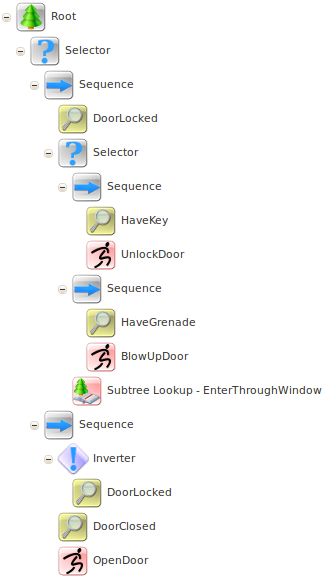
\includegraphics[width=0.7\textwidth]{./Images/ComplexEnterRoom.png}
 \caption{a complex behaviour tree}
 \label{fig:ComplexEnterRoom}
\end{figure}

\subsubsection{Execution Context}\label{sec:ExecutionContext}

All nodes in a BT have an \textit{execution context}, which is usually shared by all of them. The execution context, or \textit{context} for short, acts as a blackboard that can be used by nodes in order to write and read variables. For instance, a node may write a variable into the context, under a name \textit{MyVariable}. This variable can be read then by using its name, \textit{MyVariable}. This way, the context can be seen as a way for the nodes of a BT to communicate.

However, not always all the nodes share the same context. In general, the context of a BT is passed down from parents to children. Thus, the initial context is that of the root of the tree, which will pass it to its children. The root's children will pass the context to their own children, and so on. Nevertheless, some nodes do not pass their own context to their children, but another one instead. This new context may be empty or not, and it may be of a different type. JBT supports the following types:

\begin{itemize}
    \item Basic Context: this is just a normal context, with no especial features. It is the context that the user of the framework can create. Other types of contexts are managed through decorator tasks, and the user cannot create them.
    \item Hierarchical Context: a Hierarchical Context has another context (the \textit{input context}) as a base. When the Hierarchical Context cannot find a variable within its own set of variables, it will ask its input context for the variable. Note that the Hierarchical Context can be used to build a complex hierarchy of context: if the input context is a Hierarchical Context too, the request for the variable may go up the hierarchy until a non-Hierarchical Context is reached.
    \item Safe Context: a Safe Context has another context (the \textit{input context}) as a base. Initially, all variables are read form the input context. However, when a variable is modified, its value is not modified in the input context, but locally modified instead. From then on, the variable will be locally read (that is, from the set of variables of the Safe Context) instead of reading if from the input context. Thus, the input context is never modified. A Safe Context can be used to situations in which a certain context (the input context) must be used in read-only mode.
    \item Safe Output Context: a Safe Output Context behaves much in the same way as the Safe Context. It has another context, the \textit{input context}, as a base. However, this context also contains a set of \textit{output variables} (that is, a list of variables' names). The list of output variables represents the variables that can be modified in the input context. Variables other than those in the list of output variables will be stored locally in the set of variables of Safe Output Context, just as if it were a Safe Context. Thus, when the Safe Output Context modifies the value of a variable, it will normally set its value in a local variable (that is, a variable belonging to the Safe Output Context). However, if the variable is one of the list of output variables, the value will be set in the input context, which will therefore be modified. When retrieving variables, a variable in the list of output variables will always be retrieved from the input context. A variable that is not in the list of output variables will also be retrieved from the input context; however, when such variable is modified, the value will be retrieved from the Safe Output Context (that is, from the moment a variable that is not in the list of output variables is modified, it is managed locally).
\end{itemize}

\subsubsection{Native Tasks}

JBT offers a wide range of tasks that can be used to build behaviour trees. JBT basically implements the BT model described in \cite{Millington09}, but extended with guards.

JBT supports the following tasks:

\begin{itemize}
  \item Composite tasks: tasks with one or more children, whose execution depends on the execution of their children. The task's children are ordered.
  \begin{itemize}
    \item Sequence: task that sequentially executes all its children in order. If one fails, the Sequence task fails. If all succeeds, the Sequence task succeeds.
    \item Selector: task that sequentially executes all its children in order. If one succeeds, the Selector task succeeds. If all fail, the Selector task fails.
    \item Parallel: task that concurrently executes all its children. A Parallel task does have a \textit{parallel policy}. If the parallel task's policy is \textit{sequence}, the parallel fails if one child fails; if all succeed, then the parallel succeed. If the parallel task's policy is \textit{selector}, the parallel fails if all its children fail. If one succeeds, then the parallel also succeeds.
    \item Random Selector: task that executes all its children in a random order. If one fails, the Sequence task fails. If all succeeds, the Sequence task succeeds.
    \item Random Sequence: task that sequentially executes all its children in random order. If one succeeds, the Selector task succeeds. If all fail, the Selector task fails.
    \item Dynamic Priority List: task that executes the child with the highest priority whose guard is evaluated to true. At every AI cycle, the children's guards are re-evaluated, so if the guard of the running child is evaluated to false, it is terminated, and the child with the highest priority starts running. The Dynamic Priority List task finishes when no guard is evaluated to true (thus failing) or when its active child finishes (returning the active child's termination status).
    \item Static Priority List: task that executes the child with the highest priority whose guard is evaluated to true. Unlike the Dynamic Priority List, the Static Priority List does not keep evaluating its children's guards once a child is spawned. The Static Priority List task finishes when no guard is evaluated to true (thus failing) or when its active child finishes (returning the active child's termination status).
  \end{itemize}
  \item Decorator tasks: tasks with one child whose purpose is to alter the way other tasks behave.
  \begin{itemize}
    \item Interrupter: task that controls the termination of its child task. An Interrupter simply lets its child task run normally. If the child returns a result, the Interrupter will return it. However, the Interrupter can be asked to terminate the child task and return an specified status when done so. The task that can interrupt an Interrupter is the Perform Interruption task.
    \item Inverter: task used to invert the status code returned by its child. When the decorated task finishes, its status code gets inverted.
    \item Limit: task that limits the number of times a task can be executed. This decorator is used when a task (the child of the decorator) must be run a maximum number of times. When the maximum number of times is exceeded, the decorator will fail forever on.
    \item Repeat: task that runs its child task forever. When its child task finishes, it runs it once more.
    \item Until Fail: task that runs its child as long as it does not fail. When the child task fails, Until Fail succeeds.
    \item Succeeder: task that runts its child but, no matter its returned status, the succeeder will always succeed.
    \item Hierarchical Context Manager: task that creates a new context for its child. The context that it creates is an empty (with no variables) Hierarchical Context whose input context is the context that is passed to the Hierarchical Context Manager.
    \item Safe Output Context Manager: task that creates a new context for its child. The context that it creates is an empty (with no variables) Safe Output Context whose input context is the context that is passed to the Safe Output Context Manager.
    \item Safe Context Manager: task that creates a new context for its child. The context that it creates is an empty (with no variables) Safe Context whose input context is the context that is passed to the Safe Context Manager.
  \end{itemize}
  \item Leaf tasks: tasks with no children.
  \begin{itemize}
    \item Wait: task that keeps running for a period of time, and then succeeds. The user can specify for how long (in milliseconds) the Wait task should be running.
    \item Subtree Lookup: see the following sections to see what this node does.
    \item Perform Interruption: task that interrupts an Interrupter task.
    \item Variable Renamer: task that renames a variable in the context.
    \item Success: task that immediately succeeds.
    \item Failure: task that immediately fails.
    \item Action: generic action that is executed in the game engine.
    \item Condition: generic condition that is executed in the game engine.
  \end{itemize}
\end{itemize}

\section{Step 1: Defining Low Level Actions and Conditions}\label{sec:DefiningLowLevelActionsAndConditions}

The first step\footnote{Well, it does not necessarily have to be the first step, but we have to start at somewhere.} when creating BTs is to define the set of low level actions and conditions that the trees will be using. These actions and conditions are domain dependent, that is, they depend on the game that the trees will be run for. For instance, if we are dealing with a first person shooter (FPS from now on), then we may need actions and conditions such as those used in the trees of section \ref{sec:BTModel}. 

However, we are going to build a more complex example. Here we are going to define a behaviour tree that is able to control a Terran Marine of \starcraft, so we have to define actions and conditions that are useful for such context. The behaviour that we want to implant in the Terran Marine is as follows:

The marine is constantly checking three conditions. If there is no danger around the marine, then he just patrols around its current position. Patrolling around a position means that the marine will move randomly around a central point, and will attack whatever he finds on its way. However, if he finds himself in a low level danger situation (that is, a dangerous situation he thinks he can survive), he will try to kill whatever enemy finds dangerous. On the other hand, if he finds himself in a high level danger situation (that is, a dangerous situation he thinks he cannot survive), he will run away to the closest base.

We therefore define some actions and conditions that will be used by the BT:

\begin{itemize}
  \item Actions: 
  \begin{itemize}
	\item Attack: this action just makes the marine attacks a specific unit.
	\item Move: this action makes the marine move to a specific target position on the map.
	\item AttackMove: this action makes the marine mote to a specific target position on the map. Also, if he finds an enemy on its way, he will combat the enemy.
	\item ComputeClosestBasePosition: this action computes the position of the base that is closest to the marine.
	\item ComputeCharacterPosition: this action just computes the current position of the marine.
	\item ComputeRandomClosePosition: given a position $A$, this action computes a random position that is close to $A$.
  \end{itemize}
  \item Conditions:
  \begin{itemize}
	\item LowDanger: this condition checks if the marine is in a low danger situation.
	\item HighDanger: this condition checks if the marine is in a high danger situation.
  \end{itemize}
\end{itemize}

Actions and conditions must be defined according to the MMPM domain file format. For those unaware of what MMPM is, this does not really pose a problem, since what we are really interested in is the format that MMPM follows in order to define actions and conditions.

A MMPM domain file defines the conceptual level of a game (its \textit{domain}), by declaring what \textit{entities}, \textit{actions}, \textit{sensors} and \textit{goals} are present in the game. We will not describe all of them, but only what we need to declare actions and conditions that can be used in BTs.

A MMPM domain file has the following structure:

\begin{minted}{xml}
  <Domain package="valid Java package name">
    <ActionSet>
      <!-- Actions declaration -->
    </ActionSet>
    
    <SensorSet>
      <!-- Sensors declaration -->
    </SensorSet>

    <GoalSet>
      <!-- Goals declaration -->
    </GoalSet>

    <EntitySet>
      <!-- Entities declaration -->
    </EntitySet>
  </Domain>
\end{minted}

However, we are only interested in the set of actions and conditions, so $<GoalSet>$ and $<EntitySet>$ can be left empty (but they actually have to be present). The $<ActionSet>$ element defines the set of actions that are present in the game, which are also the set of low level actions that can be used when building BTs. An $<ActionSet>$ element contains a sequence of $<Action>$ elements, each one being an action. An $<Action>$ element has one attribute, its name (which is called $name$). The $<SensorSet>$ element defines the set of \textit{sensors} that can be used in the game. A $<SensorSet>$ element contains a sequence of $<Sensor>$ elements, each one being a sensor. A $<Sensor>$ element has two attributes: its $name$ and its $type$. In MMPM, a \textit{sensor} is an operation that queries something about the world. As a result, a sensor can return \textit{any}\footnote{Really not \textit{any}.} type of value. Here we are interested in sensors whose type is \textit{boolean} ($BOOLEAN$ in the MMPM domain file), since they represent what in BTs is known as conditions, that is, a query operation that returns either true or false. Therefore, the set of boolean sensors of the MMPM domain file is the set of conditions that can be used when building BTs. 

Both actions and sensors may have input parameters. An input parameter is a parameter that is supposed to be used by the action or sensor when running. For instance, the \textit{Move} action above does have one input parameter, which is the target position where the unit must go to. An input parameter has a name and a type. Thus, both $<Action>$ and $<Sensor>$ elements may have a sequence of $<Parameter>$ elements, each one being a parameter. Each $<Parameter>$ element has two attributes, its $name$ and its $type$. Therefore, actions and sensors have the following structure:

\begin{minted}{xml}
<Action name="MyActionName">
  <Parameter name="ParameterName1" type="ParameterType1"/>
  ...
  <Parameter name="ParameterNameN" type="ParameterTypeN"/>
</Action>

<Sensor name="MySensorName" type="BOOLEAN">
  <Parameter name="ParameterName1" type="ParameterType1"/>
  ...
  <Parameter name="ParameterNameM" type="ParameterTypeM"/>
</Sensor>
\end{minted}

MMPM supports the following types for parameter types: $FLOAT$, $BOOLEAN$, $STRING$, $INTEGER$, $DIRECTION$, $COORDINATE$, $PLAYER$, $ENTITY\_ID$ and $ENTITY\_TYPE$. This set of parameter types may seem overwhelming, which is why in general several of them are not used. $FLOAT$, $BOOLEAN$, $STRING$ and $INTEGER$ are self-explanatory. $DIRECTION$ represents an integer value, which is why, if it is used as the type of a parameter, JBT will treat it just as an integer. $COORDINATE$ represents a coordinate in an N-dimensional coordinate system. In practice, a $COORDINATE$ value is a non-empty sequence of real values (for instance, "23 -4.5 67", "-3.45 " or "12.45 -0.34 9.44 -12.3"). $PLAYER$ represents the name of a player of the game, so in practice it is treated as a string ($STRING$). $ENTITY\_ID$ represents the identifier of an entity in the game. In practice, it is treated as a string ($STRING$). $ENTITY\_TYPE$ represents the type of an entity. In practice, it is treated as a string ($STRING$).

As a consequence, the user will generally use just $FLOAT$, $BOOLEAN$, $STRING$, $INTEGER$ and $COORDINATE$, since the rest of MMPM parameter types are equivalent to $STRING$.

MMPM format, however, does not include an important parameter type, \textit{object}. In general, there will be actions and sensors will make use of input parameters of many types. In order to be able to manage a wide range of types, JBT extends the MMPM domain file format so that parameters also accept the $OBJECT$ type. An $OBJECT$ is just a variable of any type.

The MMPM domain file that defines the set of actions and conditions for the Terran Marine example is as follows:

\begin{minted}{xml}
  <Domain package="mypackage">
    <ActionSet>
      <!-- Orders the current unit to attack another unit -->
      <Action  name="Attack">
        <Parameter name="target" type="ENTITY_ID"/>
      </Action>

      <!-- Orders the current unit to go to a target position -->
      <Action  name="Move">
        <Parameter name="target" type="COORDINATE"/>
      </Action>

      <!-- Orders the current unit to go to a target position. If
      an enemy is found along the way, the unit will combat him -->
      <Action name="AttackMove">
        <Parameter name="target" type="COORDINATE"/>
      </Action>

      <!-- Orders the position of the base that is closest to the
      current unit -->
      <Action  name="ComputeClosestBasePosition"/>

      <!-- Computes the position of the current unit -->
      <Action  name="ComputeCharacterPosition"/>
      
      <!-- Computes a random position that is close to the input
      position -->
      <Action name="ComputeRandomClosePosition">
        <Parameter name="initialPosition" type="COORDINATE"/>
      </Action>
    </ActionSet>
    
    <SensorSet>
      <!-- Checks if the current unit is in a low danger situation -->
      <Sensor name="LowDanger" type="BOOLEAN"/>

      <!-- Checks if the current unit is in a high danger situation -->
      <Sensor name="HighDanger" type="BOOLEAN"/>
    </SensorSet>

    <EntitySet>
    </EntitySet>

    <GoalSet>
    </GoalSet>
  </Domain>
\end{minted}

One of the ways nodes in BTs communicate with each other is by using the execution \textit{context}: a node may write a variable into the context and another node may use it later. In this scenario it is therefore very important that nodes know the name of the variables that other nodes put into the context. In the set of actions and conditions above there are several nodes that manipulate the context. In particular:

\begin{itemize}
  \item The \textit{ComputeCharacterPosition} action writes into the context a variable of type $COORDINATE$ containing the current position of the unit. The name of such variable is \textit{CharacterPosition}.
  \item The \textit{ComputeClosestBasePosition} action writes into the context a variable of type $COORDINATE$ containing the position of the closest base. The name of such variable is \textit{ClosestBasePosition}.
  \item The \textit{ComputeRandomClosePosition} action writes into the context a variable of type $COORDINATE$ containing a random position that is close to the input position. The name of such variable is \textit{RandomClosePosition}.
  \item The \textit{LowDanger} sensor writes into the context a variable of type $ENTITY\_ID$ containing the identifier of the closest dangerous enemy. The name of such variable is \textit{LowDangerTarget}.
\end{itemize}

\section{Step 2: Implementing Low Level Actions and Conditions}\label{sec:ImplementingLowLevelActionsAndConditions}

Once that low level actions and conditions have been defined (see section \ref{sec:DefiningLowLevelActionsAndConditions}), the next step is to provide an implementation for them. JBT does not know what does an action such as \textit{ComputeCharacterPosition} or \textit{AttackMove}. Therefore, it is the user of the framework who has to tell JBT how they work.

The life cycle of actions and conditions of a BT is very simple: initially, when the flow of execution reaches the node, it is \textit{spawned}. From then on, at every \textbf{game tick}, the node is \textit{ticked}. Every time the node is ticked, it has to report about its termination status, so that the tree may evolve in case the node has finished. As a result, the programmer will have to define how all the domain dependent actions and conditions behave when they are spawned and ticked.

Actions and conditions are each represented by two classes of the JBT Core, \textit{jbt.model.task.leaf.action.ModelAction.java} and \textit{jbt.execution.task.leaf.action.ExecutionAction.java} in the case of actions, and \textit{jbt.model.task.leaf.condition.ModelCondition.java} and \textit{jbt.execution.task.leaf.condition.ExecutionCondition.java} in the case of conditions. Domain dependent actions such as the ones defined above must extend these classes in order for JBT to know how to work with them.

In JBT there are two classes for every type of node. Remember from section \ref{sec:ModelIndependentFromExecution} that in JBT there are two types of BTs, the \textit{Model BT} and the \textit{Execution BT}. The Model BT is composed of \textit{model tasks\footnote{Remember that in BT terminology, a task and a node are the same thing.}}, while the Execution BT is composed of \textit{execution tasks}. It is the execution tasks that define how the tasks work, that is, how they behave when they are spawned and ticked. In the case of actions and conditions, the four classes presented above are the base classes for their respective representation as model tasks and execution tasks.

JBT Core offers a tool that semi-automatize the task of creating all the classes from each action and condition of the MMPM domain file. It is the Java class \textit{jbt.tools.btlibrarygenerator.ActionsAndConditionsGenerator.java}.

For every MMPM action, ActionsAndConditionsGenerator creates two classes: one extending ModelAction, which conceptually represents the action, and another one extending ExecutionAction, which represents how the action actually works -whose abstract methods must be completed in order for the action to perform any task at all. We will explain this later-.

Also, for every MMPM boolean sensor, two classes are created: one extending ModelCondition, which conceptually represents the condition (sensor), and another one extending ExecutionCondition, which represents how the condition actually works -whose abstract methods must be completed in order for the condition to perform any task at all. We will explain this later-.

The syntax of the program is as follows:

\begin{verbatim}
ActionsAndConditionsGenerator -c configurationFile [-r relativePath] [-o] 
\end{verbatim}

Where \verb@configurationFile@ is an XML file that contains all the information required to run the application. The syntax of such file is:

\begin{minted}{xml}
<Configuration>
  <DomainFile>MMPMDomainFile1</DomainFile>
  <DomainFile>MMPMDomainFile2</DomainFile>
  ...
  <DomainFile>MMPMDomainFileN</DomainFile>
  
  <ModelActionsPackage>Name of the package for generated model
  action classes</ModelActionsPackage>
  
  <ModelConditionsPackage>Name of the package for generated model 
  condition classes</ModelConditionsPackage>
  
  <ModelActionsOutputDirectory>Name of the directory where model 
  actions are created</ModelActionsOutputDirectory>
  
  <ModelConditionsOutputDirectory>Name of the directory where model 
  conditions are created</ModelConditionsOutputDirectory>
  
  <ExecutionActionsPackage>Name of the package for generated 
  execution action classes</ExecutionActionsPackage>
  
  <ExecutionConditionsPackage>Name of the package for generated
  execution condition classes</ExecutionConditionsPackage>
  
  <ExecutionActionsOutputDirectory>Name of the directory where 
  execution actions are created</ExecutionActionsOutputDirectory>
  
  <ExecutionConditionsOutputDirectory>Name of the directory where 
  execution conditions are created</ExecutionConditionsOutputDirectory>
</Configuration>
\end{minted}

The order in which the elements are specified is not relevant. If the input files do contain only actions, parameters related to conditions may not be specified, and vice versa.

The -r option is used to add a path to the beginning of the files listed in the configuration file; as a result, each file is considered to be placed at the path specified in the -r option. The -r option may not be specified, in which case the files are considered to be at the current execution directory.

The -o option (standing for \textit{overwrite}) is either is specified or not. If it is not specified, generated output files will not overwrite any existing file in the file system, and as a result, the corresponding class file will not be produced in case there is a file with the same name in the file system. If the option -o is specified, then generated output files will overwrite any file in the file system whose name matches.

So, in brief, this program parses a MMPM domain file and, for each action and boolean sensors produces the JBT classes that are required to run such actions and conditions in a BT. In particular, the created execution classes define what they will do when spawned and ticked.

The generated ModelAction and ModelCondition classes are complete, so they do not need to be modified after being created by the ActionsAndConditionsGenerator. However, the ExecutionAction and ExecutionCondition generated classes contain a set of abstract method that must be implemented according to the semantics of the respective actions and conditions, so that they do what they are expected to do. This is the only step that must be done in order for JBT to be able to work with the low level actions and conditions provided by the user.

In particular, the abstract methods that must be implemented are:

\begin{minted}{java}
protected void internalSpawn();
protected Status internalTick();
protected void internaTerminate();
protected void restoreState(ITaskState state);
protected ITaskState storeState();
protected ITaskState storeTerminationState(); 
\end{minted}

\textit{internalSpawn()} and \textit{internalTick()} are the most important methods, so they should be well implemented.

\textit{internalSpawn()} represents the spawning process of the task (action or condition). When the flow of execution of the tree reaches the task, \textit{internalSpawn()} gets called. Therefore, this method must be defined so that it starts the process associated to the task. For instance, the \textit{internalSpawn()} method of the \textit{Move} action above should order the current unit to go to the target position; the \textit{internalSpawn()} method of the \textit{Attack} action above should order the current unit to attack the target enemy. 

The automatically generated skeleton contains an initial implementation of the \textit{internalSpawn()} method, which is as follows:

\begin{minted}{java}
protected void internalSpawn() {
  /*
   * Do not remove this first line unless you know what it does and you
   * need not do it.
   */
  this.getExecutor().requestInsertionIntoList(
    jbt.execution.core.BTExecutor.BTExecutorList.TICKABLE, this);

  /* TODO: this method's implementation must be completed. */
  System.out.println(this.getClass().getCanonicalName() + " spawned");
}     
\end{minted}

This initial definition contains a very important aspect of the execution process of the task. As it is said in the comments, the first line should not be removed unless the user knows what it does and he thinks it is not necessary to do it. What that line does is to request that the task be inserted into the list of tickable nodes (section \ref{sec:ModelDrivenByTicks}). Since in general this is what we want the task to do (because we want the task to receive ticks), \textbf{that line should not be removed}.

When implementing all these abstract methods, the user may access the execution context of the task by calling \textit{this.getContext()}. That method just returns the context of the task as an \textit{IContext} object. The \textit{IContext} interface defines two main methods, one for reading a variable from the context, and another one for writing a variable into the context:

\begin{minted}{java}
public interface IContext {
  /**
   * Returns the value of a variable whose name is <code>name</code>, or null
   * if it is not found.
   */
  public Object getVariable(String name);

  /**
   * Sets the value of a variable. If the variable already existed, its value
   * is overwritten. <code>value</code> may be null in order to clear the
   * value of the variable.
   */
  public boolean setVariable(String name, Object value);
  ...
}
\end{minted}

Remember that MMPM domain files also let the designer specify input parameters for actions and sensors. These are parameters that actions and sensors are supposed to use when running. The generated JBT ExecutionAction and ExecutionCondition classes include \textit{getter} methods for such input parameters. As a result, the programmer will be able to access the value of the input parameters in the abstract methods he has to implement, by using the getter methods. The value for the input parameters are either retrieved from the execution context(IContext) or directly provided at construction time, but these details are hidden from the programmer that implements the action or condition (he should just use the getter methods to retrieve whatever input parameters may be needed). For instance, for the \textit{Attack} action, the next getter method is created:

\begin{minted}{java}
/**
  * Returns the value of the parameter "target", or null in case it has not
  * been specified or it cannot be found in the context.
  */
public java.lang.String getTarget(){...}
\end{minted}

Thus, in the implementation of all the abstract methods, the user should use this \textit{getTarget()} method if he wanted to retrieve the identifier of the target unit to attack. This whole thing about the getter methods may be a little bit confusing at first. However, bear in mind that when the user creates a behaviour tree (which we will explain later), he can either specify that the input parameter of a task must be retrieved from a variable of the context, or provide an actual value for the parameter. When the task is spawned and run, it does not really care about where the parameter comes from as long as there is a value that it can use. The generated getter methods hide these details, so no matter where the parameter comes from (either from the context or from an actual value provided by the user when he created the BT), it just provides the value that the task expects to use.

Once the task has been spawned, it will be ticked whenever the BT gets ticked. The ticking process is performed by the \textit{internalTick()} method. Thus, from the moment the task gets spawned, at every tick, \textit{internalTick()} will be called. 

\textit{internalTick()} is in charge of keeping track of the termination status of the task. If the task has not finished yet when \textit{internalTick()} is called, then it must return the termination status \textit{Status.RUNNING}. If the task has finished successfully, then the method should return the termination status \textit{Status.SUCCESS}. If the task has finished unsuccessfully, then the method should return \textit{Status.FAILURE}. For instance, the \textit{internalTick()} method of the \textit{Move} action of our Terran Marine example should check if the unit has arrived at the target position. If it has not, then \textit{Status.RUNNING} should be returned. If the unit has arrived at the target position, then \textit{Status.SUCCESS} should be returned. Finally, y for some reason the action could not be completed (for instance because the target position is unreachable), then \textit{Status.FAILURE} should be returned. Note that, even though the \textit{Status} enum has more values other than \textit{SUCCESS}, \textit{FAILURE} and \textit{RUNNING}, the \textit{internalTick()} method must return only one of these three. Doing otherwise will throw an exception.

One of the ideas behind the \textit{driven by ticks} architecture is that, when the tree is ticked, it should not take very long for it to return, so \textit{internalSpawn()} and \textit{internalTick()} are supposed to return very quickly. However, sometimes tasks perform computationally expensive processes. In that case, instead of performing the expensive computation inside the \textit{internalSpawn()} method of the task, it should be performed in another execution thread. When \textit{internalSpawn()} is called, it should create another thread that carries out the computation. On the other hand, the \textit{internalTick()} method would query the thread to check if its computation has finished or not, and return \textit{Status.RUNNING}, \textit{Status.SUCCESS} or \textit{Status.FAILURE} accordingly.

The \textit{internalTerminate()} method is not so important. Sometimes, when a BT is running, some of its tasks get abruptly interrupted. This happens for instance when one of the children of a parallel task (which is following the \textit{sequence policy}) fails. When that happens, all of its children, which were being concurrently evaluated, get terminated, so they must stop running. Other scenario in which this happens is when a perform interruption task interrupts an interrupter. In that case, the interrupter and its child stop running.

It is for cases like these that the \textit{internalTerminate()} method is defined. The \textit{internalTerminate()} method must make the task stop running. For instance, in the case of the \textit{Move} action, it should order the unit to stop moving. Moreover, if the task started some other thread to perform some computations, it should stop it. In general, when the \textit{internalTerminate()} is called, the task should stop running and should also free whatever resources it acquired.

With respect to the \textit{storeState()}, \textit{storeTermination} and \textit{restoreState(ITaskState state)}, they are related to \textit{persistent tasks}. Some tasks in BTs are persistent in the sense that, after finishing, if they are spawned again, they should remember past information. Take for example the Limit task. A Limit task allows to run its child node only a certain number of times (for example, 5). After being spawned, it has to remember how many times it has been run so far, so that, once the threshold is exceeded, it fails. In general, it could be said that some tasks need to retain some persistent information to be used in the future when the task is spawned again.

All the persistent information of a task should be saved into an \textit{ITaskState} object. The ITaskState interface represents a collection of variables that can be accessed:

\begin{minted}{java}
public interface ITaskState {
  /* Returns the value of a state variable by its name. */
  public Object getStateVariable(String name);
} 
\end{minted}

When a task finishes, (it returns \textit{Status.SUCCESS} or \textit{Status.FAILURE} in \textit{internalTick()}), the \textit{storeState()} method is automatically called by the framework. This method should then create and return an \textit{ITaskState} object containing all the persistent information that the task may need if it is spawned again in the future. If no persistent information is needed, then \textit{null} must be returned. An \textit{ITaskState} object is just a collection of variables that can be retrieved by name. In order for the user to create \textit{ITaskState} objects, he can make use of the factory class \textit{jbt.execution.core.TaskStateFactory}.

It also may be the case that a task that is abruptly terminated (\textit{internalTerminate()} is called) needs to store persistent information. If that is the case, then \textit{storeTerminationState()} is automatically called by the framework, instead of \textit{storeState()}. \textit{storeTerminationState()} follows the same semantics as \textit{storeState()}.

The persistent information that a task stores via its \textit{storeState()} and \textit{storeTerminationState()} methods is restored via the \textit{restoreState(ITaskState state)} method. This method is called just before the task is spawned (that is, before calling \textit{internalSpawn()}). In \textit{restoreState(ITaskState state)} the task should analyse the input \textit{ITaskState} object and restore whatever information it contains (if \textit{null}, then it means that there is no past information to remember).

In the case of the \textit{Move} action of the Terran Marine example, the \textit{storeState()}, \textit{storeTerminationState()} and \textit{restoreState(ITaskState state)} methods are empty.

As a final example on implementing low level actions and conditions, lets follow the whole process for the few actions and conditions defined in the domain explained in section \ref{sec:DefiningLowLevelActionsAndConditions}.

Let us suppose that the MMPM domain file is stored in the file \textit{TerranMarineDomain.xml}. Then, the ActionsAndConditionsGenerator application could be run with the next configuration file (stored in \textit{configurationFile.xml}):

\begin{minted}{xml}
<Configuration> 
  <DomainFile>TerranMarineDomain.xml</DomainFile>
  <ModelActionsPackage>bts.actions</ModelActionsPackage>
  <ModelConditionsPackage>bts.conditions</ModelConditionsPackage>
  <ModelActionsOutputDirectory>src/bts/actions
  </ModelActionsOutputDirectory>
  <ModelConditionsOutputDirectory>src/bts/conditions
  </ModelConditionsOutputDirectory>
  <ExecutionActionsPackage>bts.actions.execution
  </ExecutionActionsPackage>
  <ExecutionConditionsPackage>bts.conditions.execution
  </ExecutionConditionsPackage>
  <ExecutionActionsOutputDirectory>src/bts/actions/execution
  </ExecutionActionsOutputDirectory>
  <ExecutionConditionsOutputDirectory>src/bts/conditions/execution
  </ExecutionConditionsOutputDirectory>
</Configuration>
\end{minted}

Let us suppose that the ActionsAndConditionsGenerator is called with the following arguments:

\begin{verbatim}
ActionsAndConditionsGenerator -c configurationFile.xml -r /home/outputDirectory
\end{verbatim}

Then, the ActionsAndConditionsGenerator will parse the domain file \textit{/home/outputDirectory/\-TerranMarine.xml}, and it will create output classes for each action and boolean sensor in the domain file, which will be stored in the corresponding files. For instance, for the \textit{Attack} action, two classes will be created, \textit{/home/outputDirectory/src/bts/actions/Attack.java} (the model task class) and \textit{/home/outputDirectory/src/bts/actions/execution/Attack.java} (the execution task class). For the boolean \textit{LowDanger} sensor, two classes will be created, \textit{/home/outputDirectory/src/bts/conditions/LowDanger.java} (the model task class) and \textit{/home/outputDirectory/src/bts/conditions/execution/LowDanger.java} (the execution task class). Then we should implement the abstract methods of all the execution classes. For instance, the implementation of the \textit{Move.java} execution class may be like this:

\begin{minted}{java}
/** ExecutionAction class created from MMPM action Move. */
public class Move extends jbt.execution.task.leaf.action.ExecutionAction {
  ...
  /**
   * Returns the value of the parameter "target", or null if not found
   * anywhere.
   */
  public float[] getTarget() {
    /* Whatever has been automatically generated. */
    ...
  }

  protected void internalSpawn() {
    this.getExecutor().requestInsertionIntoList(
            jbt.execution.core.BTExecutor.BTExecutorList.TICKABLE, this);

    /* 
     * Retrieve the identifier of the entity (Terran Marine) running 
     * this action from the context. Here we are supposing that the 
     * context will contain it.
     */
    String currentEntityID = (String) this.getContext().
                                      getVariable("CurrentEntityID");

    /* 
     * Now we assume that there is a generic "Game Engine" that can
     * be used to send generic orders to units of the game. Note that, in
     * order to retrieve the target position, we use the automatically
     * generated getter method.
     */
    GameEngine.sendMoveOrder(currentEntityID, this.getTarget());
  }

  protected jbt.execution.core.ExecutionTask.Status internalTick() {
    /*
     * In this method we will just check whether the unit has reached the
     * target position. If the target position is unreachable, then 
     * Status.FAILURE is returned. Otherwise, if the unit has reached the
     * target position, Status.SUCCESS is returned. Otherwise,
     * Status.RUNNING is returned.
     */
    String currentEntityID = (String) this.getContext().
                                      getVariable("CurrentEntityID");

    if(!Util.reachablePosition(currentEntityID, this.getTarget())){
      return Status.FAILURE;
    }

    float[] currentPosition = GameEngine.getPosition(currentEntityID);
    float[] targetPosition = this.getTarget();

    if(Math.distance(currentPosition, targetPosition) < 0.5){
      return Status.SUCCESS;
    }
    else{
      return Status.RUNNING;
    }
  }

  protected void internalTerminate() {
    /* We just order the unit to stop. */
    String currentEntityID = (String) this.getContext().getVariable(
            Constants.CONTEXT_CURRENT_ENTITY);

    GameEngine.stopUnit(currentEntityID);
  }

  protected void restoreState(jbt.execution.core.ITaskState state) {
    /* Does nothing. */
  }

  protected jbt.execution.core.ITaskState storeState() {
    /* No persistent state information to return. */
    return null;
  }

  protected jbt.execution.core.ITaskState storeTerminationState() {
    /* No persistent state information to return. */
    return null;
  }
}
\end{minted}

\section{Step 3: Creating BTs with the JBT Editor}\label{sec:CreatingBTsWithTheJBTEditor}

Once that the domain dependent actions and conditions of the game have been defined and a JBT implementation for them has been provided, the next steps are quite easy to follow. 

It is now when the user should define the behaviour trees to use in the game. Following our Terran Marine example, we will define several trees that implement the behaviour that we described in section \ref{sec:DefiningLowLevelActionsAndConditions}.

Behaviour trees are first described in XML files. Here we are not going to describe the XML format that JBT understands, since we discourage the user from writing them in plain text. Instead, we propose to use the JBT Editor (composed of the two projects under the ``./JBTEditor'' directory of the repository), a GUI application through which it is really easy to define behaviour trees.

The JBT Editor is an Eclipse RCP application. As such, it must be run under the Eclipse SDK environment or use the executable files provided for each platform. When opening if from Eclipse, you have to open the project \textit{jbt.tools.bteditor}, and then open the file \textit{bteditor.product} with the Product Configuration Editor. Once it has been opened, go to the ``Overview'' page, and click on ``Launch an Eclipse application''. A window like that of figure \ref{fig:JBTEditor} should show up.

\begin{figure}
 \centering
 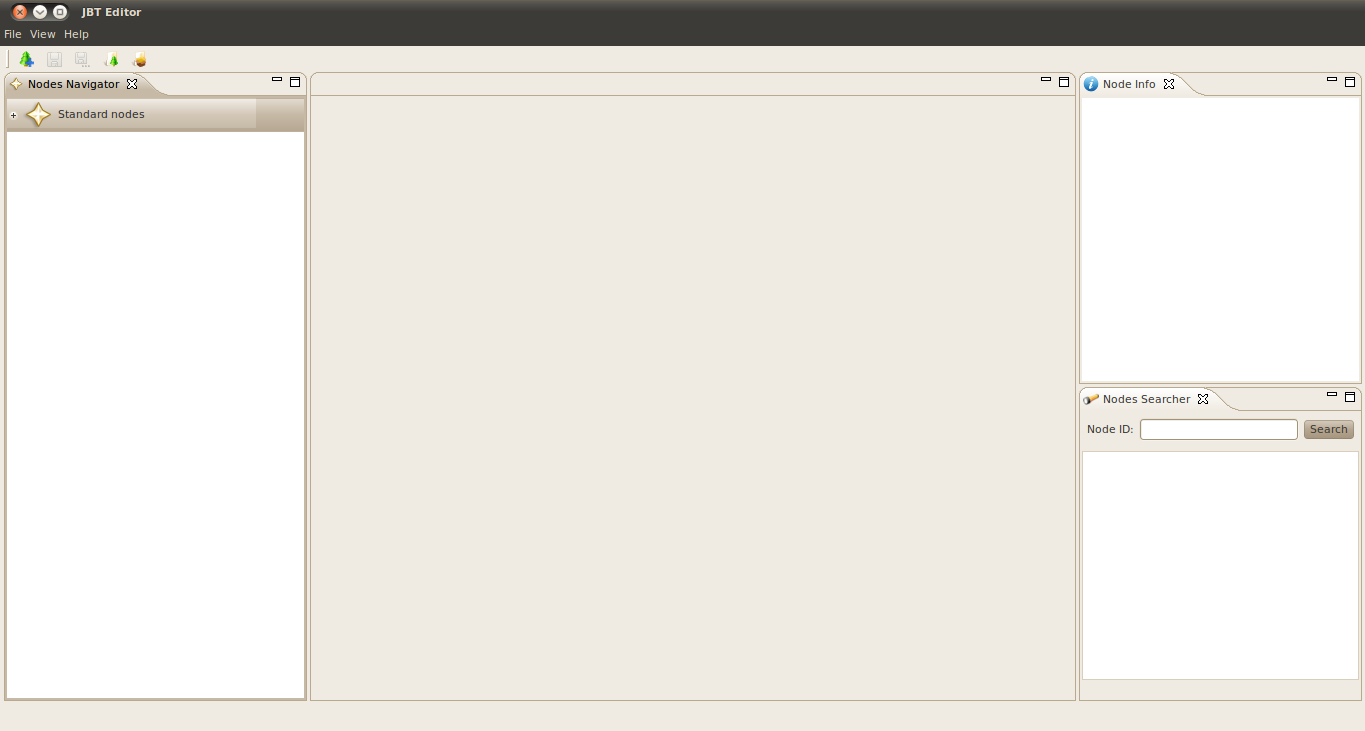
\includegraphics[width=\textwidth]{./Images/JBTEditor.png}
 \caption{JBT Editor after being opened}
 \label{fig:JBTEditor}
\end{figure}

The JBT Editor is a very simple tool, so learning how to use it should not take very long.

In order to create a new BT, just click on the ``new BT'' icon or select ``File->New BT''. A new editor should open up showing an empty BT (that is, a tree containing only a single node, the root of the tree. To the right of the window there is a tree-like menu (the \textit{Nodes Navigator}) where the user can select nodes to build the tree. In order to add a node to a tree, just drag it from the Nodes Navigator and drop it onto whatever node of the tree to insert it as a child or sibling of the target node. The root node can have only one child. However, other nodes, such as sequences or selectors may have many of them. Decorators can have only one child, and leaf nodes do not have any children.

By using the set of provided standard nodes of the Nodes Navigator, the user can build complex behaviour trees. However, in order to build really useful trees, the user must use the domain-dependent actions and conditions from the game. The JBT Editor lets the user load a MMPM domain file as described in section \ref{sec:DefiningLowLevelActionsAndConditions}. Just click on the ``Load MMPM Domain'' or select ``File->Load MMPM Domain'' and select the file that contains the low level actions and conditions. After doing so, the Nodes Navigator will be added a new entry for the actions and conditions within the domain file, which the user will be able to use when building BTs.

For instance, if we load the domain file described in section \ref{sec:DefiningLowLevelActionsAndConditions}, we get the actions and conditions shown in figure \ref{fig:LoadedDomain}.

\begin{figure}
 \centering
 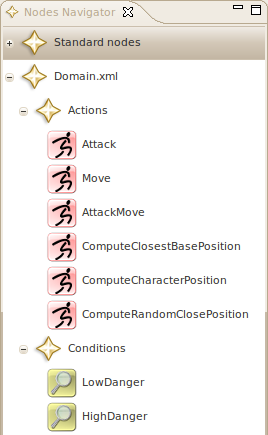
\includegraphics[width=0.4\textwidth]{./Images/LoadedDomain.png}
 \caption{The Nodes Navigator after loading the domain file}
 \label{fig:LoadedDomain}
\end{figure}

The JBT Editor lets the user specify values for the input parameters of nodes. By double clicking on a node that has input parameters, a dialog where the user can specify values for the input parameters. For instance, if the AttackMove action is double clicked, then the dialog of figure \ref{fig:InputParameterDialog} is shown. In the dialog the user can specify a value for the parameter ``target'', whose type is $COORDINATE$. Thus, the text field only supports values such as ``45 62'' or ``10 -3 45''. As we mentioned in section \ref{sec:ImplementingLowLevelActionsAndConditions}, when building a BT, the user can specify whether the input parameters of actions and conditions are retrieved from the context or an actual value is provided at construction time. The ``From context'' check box lets the user specify if the parameter has to be retrieved from the context or not. If the check box is not ticked, then the user must provide a value for the parameter in the text field. However, if the check box is ticked, then what the user does is to specify the name of the context's variable where the value of the parameter will be retrieved from.

\begin{figure}
 \centering
 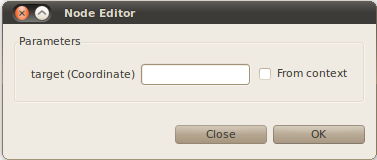
\includegraphics[width=0.4\textwidth]{./Images/InputParameterDialog.png}
 \caption{The dialog for editing the input parameters of the AttackMove action}
 \label{fig:InputParameterDialog}
\end{figure}

For instance, in figure \ref{fig:ParameterNotFromContext} the user has specified a value (``12 34 4.5'') for the input parameter ``target'' of the AttackMove action. However, in figure \ref{fig:ParameterFromContext} the user has indicated that the value of the input parameter ``target'' will be retrieved from the variable ``TargetVariable'' of the context.

\begin{figure}
 \centering
 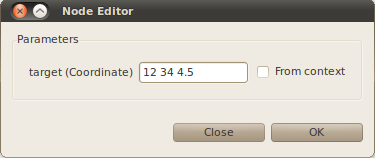
\includegraphics[width=0.4\textwidth]{./Images/ParameterNotFromContext.png}
 \caption{A parameter for which an actual value is provided}
 \label{fig:ParameterNotFromContext}
\end{figure}

\begin{figure}
 \centering
 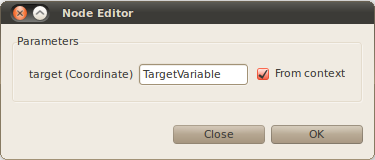
\includegraphics[width=0.4\textwidth]{./Images/ParameterFromContext.png}
 \caption{A parameter whose value will be retrieved from the context}
 \label{fig:ParameterFromContext}
\end{figure}

Once the BT has been completed, the user can save it as an XML file. In order to do so, just click on the ``Save'' or ``Save As'' icons (or select ``File->Save'' or ``File->Save As'') and enter a file name.

When saving a BT, the JBT Editor checks if the structure of the tree is correct. If not, incorrect nodes are highlighted in red color and an explanation for the error is shown in the \textit{Node Info} view (to the right of the window) when the node is selected.

Also note that a name for the BT must be provided. The name of a BT is specified in the root node of the tree. When the root is double clicked, a dialog appears that lets the user assign the tree a name. BTs' names are very important, because it is the way that trees are referenced. In particular, names are essential in terms of reusability. For instance, the \textit{Subtree Lookup} task simulates a particular BT, and the way that the Subtree Lookup knows what BT to simulate is by providing the name of the tree.

Let us now design the BT that implements the Terran Marine behaviour that we described in section \ref{sec:DefiningLowLevelActionsAndConditions}. An initial implementation for such tree could be that of figure \ref{fig:InitialTerranMarineBT}. 

\begin{figure}
 \centering
 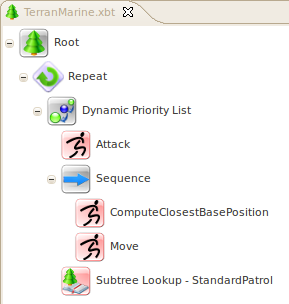
\includegraphics[width=0.4\textwidth]{./Images/InitialTerranMarineBT.png}
 \caption{Initial tree for the Terran Marine behaviour}
 \label{fig:InitialTerranMarineBT}
\end{figure}

The behaviour is pretty simple: the tree is always executing (see the \textit{Repeat} node) a \textit{Dynamic Priority List} (DPL) that is constantly checking three conditions:

\begin{itemize}
  \item If the current unit is in a low danger situation, then the unit is ordered to attack the closest dangerous enemy. This is represented by the first child of the DPL.
  \item If the current unit is in a high danger situation, then the unit runs away to the closest base. This is represented by the second child of the DPL (the Sequence).
  \item Finally, if none of the above conditions are met, the unit just ``patrols''. This is represented by the third child of the DPL, the Subtree Lookup node (we will further explain this later).
\end{itemize}

There are some details that must still be defined though. So far, the tree does not provide a way of checking the three conditions above. In order to do so, we can make use of guards, since the DPL interacts with children that have guards defined. In order to add a guard to a node, just right click on the node and select ``Edit Guard''. A dialog should appear that lets the user edit the guard of the node.

In JBT, guards are represented by BTs. In particular, a guard can be a single node or a complete and correct BT. When the user clicks on ``Add simple guard'', a dialog lets the user select a single leaf node (action, condition or a standard leaf node) to be used as a guard. If the user clicks on the ``Add complex guard'', however, a new editor is opened so the user can create a complete BT to be used as the node's guard. 

In our example, the guard of the \textit{Attack} action is just the condition \textit{LowDanger}. Therefore, we have to click on the ``Add simple guard'' button and select the ``LowDanger'' task from the list, as shown in figure \ref{fig:LowDangerGuard}. Note that after inserting the guard, a small shield icon will appear on top of the node that has been added a guard.

\begin{figure}
 \centering
 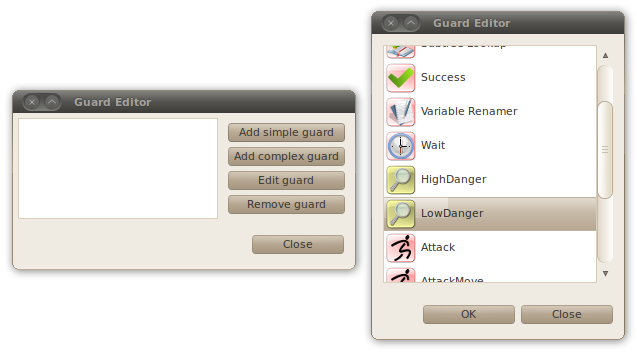
\includegraphics[width=0.55\textwidth]{./Images/LowDangerGuard.png}
 \caption{Selecting a guard for the \textit{Attack} node}
 \label{fig:LowDangerGuard}
\end{figure}

In the case of the \textit{Sequence} node, its guard is just the condition \textit{HighDanger}, so we add it just the same way. Now we have to define the input parameters of the tasks.

First of all there is the \textit{Attack} node. The intended behaviour is for the soldier to attack the closest unit once that the \textit{LowDanger} condition has been triggered. Thankfully, \textit{LowDanger} writes into the context the identifier of the closest entity (as we described in section \ref{sec:DefiningLowLevelActionsAndConditions}), in a variable with name \textit{LowDangerTarget}. Therefore, the input parameter of \textit{Attack} should be as represented in figure \ref{fig:AttackParameter}, since the value of the input parameter of the \textit{Attack} action is present in a variable of the context whose name is \textit{LowDangerTarget}.

\begin{figure}
 \centering
 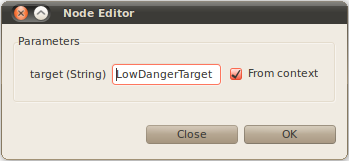
\includegraphics[width=0.4\textwidth]{./Images/AttackParameter.png}
 \caption{The input parameter of \textit{Attack}}
 \label{fig:AttackParameter}
\end{figure}

With respect to the \textit{Move} action, the idea is that the unit goes to the closest base. Since the position of the closest base has been computed by the \textit{ComputeClosestBasePosition} action and written into the context in a variable with name \textit{ClosestBasePosition}, then the input argument of \textit{Move} must be read from the context and its value must be the variable name \textit{ClosestBasePosition}.

Now let us look at the final part of the tree. When none of the danger conditions are met, the marine has to patrol around its current position. Since \textit{patrolling} is a complex task that may be reused in another trees, we decide to put it into another BT and reuse of from the Terran Marine BT. This is accomplished by the Subtree Lookup task, whose input parameter is set to \textit{StandardPatrol}. \textit{StandardPatrol} is the name of the tree that will implement the patrol behaviour.

The tree of figure \ref{fig:StandardPatrol} implements the patrol behaviour. Initially, the current position of the unit is computed by the \textit{ComputeCharacterPosition} action. This position is written into the variable \textit{CharacterPosition} of the context, as we mentioned in section \ref{sec:DefiningLowLevelActionsAndConditions}. From then on, the is a forever loop (Repeat node) that constantly computes a random position that is close to the one computed by the \textit{ComputeCharacterPosition} task, and then orders the unit to \textit{AttackMove} to that target position. It is important to note that the tree must have a name (it is set in the root of the tree), in this case \textit{StandardPatrol}, which is the name that was used in the \textit{SubtreeLookup} task of the Terran Marine BT.

\begin{figure}
 \centering
 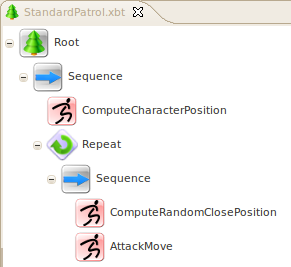
\includegraphics[width=0.4\textwidth]{./Images/StandardPatrol.png}
 \caption{The BT for the Standard Patrol behaviour}
 \label{fig:StandardPatrol}
\end{figure}

Note that a name for the Terran Marine BT must be provided, so we will assume that its name is \textit{TerranMarine}.

\section{Step 4: Creating a Java Declaration of the BTs}

Once our BTs have been defined in the XML format of the JBT Editor, the next steps are quite easy. Actually, there is no more complex work to be done by the user from now on.

So far we have provided a definition and implementation of domain dependent low level actions and conditions. We have also defined our BTs and stored them in XML files using the JBT Editor. The next step is to provide a Java implementation of the trees so that JBT can actually run them.

This step is automatically performed by the JBT Core. The JBT Core has an application, the \textit{jbt.tools.btlibrarygenerator.BTLibraryGenerator.java}, that basically takes the XML definition of some BTs and creates a .java file that contains the implementation of such trees.

In JBT, BTs are grouped together in BT libraries. A BT library is just a collection of BTs that can be retrieved by name (actually, the name that is specified for the tree in the JBT Editor). A BT library is implemented by the \textit{IBTLibrary} interface. This interface just represents a set of BTs that can be retrieved by name:

\begin{minted}{java}
public interface IBTLibrary extends Iterable<Pair<String, ModelTask>> {
    /* Returns the BT of name name, or "null" if not found. */
    public ModelTask getBT(String name);
}
\end{minted}

Note that, in JBT, a Model BT (see section \ref{sec:ModelIndependentFromExecution}) is represented by the abstract class \textit{ModelTask}. Thus, when we ask an \textit{IBTLibrary} to give us a BT by its name, it just retrieves the Mode BT that represents the tree, which is represented by a \textit{ModelTask}.

What the BTLibraryGenerator does is to automatically create a BT library, that is, a class that implements the \textit{IBTLibrary} interface, that can be used to retrieve the BTs defined in the XML files. In particular, given a set of behaviour trees specified in XML files and the MMPM definition of the low level actions and conditions that are used in the trees, it creates the corresponding Java class.

The syntax of this program is as follows:

\begin{verbatim}
BTLibraryGenerator -c configurationFile [-r relativePath] [-o] 
\end{verbatim}

Where \verb@configurationFile@ is an XML file that contains all the information required to run the application. The syntax of such a file is:

\begin{minted}{xml}
<Configuration>
  <BTLibrary>
    <BTFile>BTFile1</BTFile>
    <BTFile>BTFile2</BTFile>
    ...
    <BTFile>BTFileN</BTFile>    
 
    <DomainFile>MMPMDomainFile1</DomainFile>
    <DomainFile>MMPMDomainFile2</DomainFile>
    ...
    <DomainFile>MMPMDomainFileN</DomainFile>
  
    <ModelActionsPackage>Name of the package where model action 
    classes are placed</ModelActionsPackage>
  
    <ModelConditionsPackage>Name of the package where model 
    condition classes are placed</ModelConditionsPackage>
  
    <LibraryClassName>Name of the class that is going to be 
    created</LibraryClassName>
  
    <LibraryPackage>Name of the package for the generated BT 
    library</LibraryPackage>
    
    <LibraryOutputDirectory>Name of the directory where the 
    generated library is going to be stored</LibraryOutputDirectory>
  </BTLibrary>
  
  <BTLibrary>
  ...
  </BTLibrary>

  ...
</Configuration>
\end{minted}

The order in which the elements are specified is not relevant.

In the file the user can define several BT libraries, each one within the \textit{BTLibrary} element. For each BT library defined in a \textit{BTLibrary} element, the program will produce an output file (class implementing the \textit{IBTLibrary} interface) for the library.

The -r option is used to add a path to the beginning of the files listed in the configuration file; as a result, each file is considered to be placed at the path specified in the -r option. The -r option may not be specified, in which case the files are considered to be at the current execution directory.

The -o option (standing for overwrite) is either is specified or not. If it is not specified, the generated output files will not overwrite any existing file in the file system, and as a result, a behaviour tree library may not be produced in case there is a file with the same name in the file system. If the option -o is specified, then generated output files will overwrite any file in the file system whose name matches.

In the Terran Marine example, we want to create a BT library that contains the two BTs that we created in section \ref{sec:CreatingBTsWithTheJBTEditor}. Let us suppose that the tree defining the Terran Marine behaviour was stored in the file \textit{TerranMarine.xbt}, and that the tree defining the patrol behaviour was stored in the file \textit{StandardPatrol.xbt}. Then, we could use the following configuration file to produce the BT library:

\begin{minted}{xml}
<Configuration>
  <BTLibrary>
    <BTFile>TerranMarine.xbt</BTFile>
    <BTFile>StandardPatrol.xbt</BTFile>
    <LibraryClassName>TerranMarineBTLibrary</LibraryClassName>
    <LibraryPackage>bts.btlibrary</LibraryPackage>
    <LibraryOutputDirectory>src/bts/btlibrary</LibraryOutputDirectory>
    <DomainFile>TerranMarineDomain.xml</DomainFile>
    <ModelActionsPackage>bts.actions</ModelActionsPackage>
    <ModelConditionsPackage>bts.conditions</ModelConditionsPackage>
  </BTLibrary>
</Configuration>
\end{minted}

Where note that \textit{TerranMarineDomain.xml} is the domain file that we created in section \ref{sec:DefiningLowLevelActionsAndConditions}. The \textit{ModelActionsPackage} and \textit{ModelConditionsPackage} must also be those specified in the configuration file of the ActionsAndConditionsGenerator.

So now let us suppose that the configuration file above is stored in a file called \textit{BTConfigurationFile.xml}. The BTLibraryGenerator may be called with the following arguments:

\begin{verbatim}
BTLibraryGenerator -c BTConfigurationFile.xml -r /home/outputDirectory
\end{verbatim}

Then, the BTLibraryGenerator will parse the configuration file and it will realize that it has to create just one BT library (the only \textit{BTLibrary} element in the configuration file). It will then parse the XML files of the trees that the library will contain (\textit{TerranMarine.xbt} and \textit{StandardPatrol.xbt}) and finally will create an BT library class named \textit{TerranMarineBTLibrary}, which will be placed in the output directory \textit{home/outputDirectory/stc/bts/btlibrary}. Our purpose here is not to analyse all the details of the produced class, but just point out that it can be used through the public interface that it implements (the \textit{IBTLibrary} mentioned earlier). The class \textit{TerranMarineBTLibrary} will contain both trees, so

\begin{minted}{java}
getBT("TerranMarine");
\end{minted}

will return the tree implementing the Terran Marine behaviour, and

\begin{minted}{java}
getBT("StandardPatrol");
\end{minted}

will return the tree implementing the patrol behaviour.

The way we can actually run these trees is explained in section \ref{sec:RunningTheBehaviourTrees}.

\section{Step 5: Running the Behaviour Trees}\label{sec:RunningTheBehaviourTrees}

So that is almost all. The last step is to run the trees that have been put into one or several BT libraries.

The way BTs are run in JBT is really simple, and follows the ideas mentioned in sections \ref{sec:ModelDrivenByTicks}, \ref{sec:ModelIndependentFromExecution} and \ref{sec:Architecture}.

Basically, the IBTLibrary is used to retrieve Model BTs. Once a Model BT has been retrieved, a BT Executor must be created to run it. The BT Executor must be fed with an initial context that the BT will use when running\footnote{Remember that the BT that actually runs is the Execution BT, but that detail is of no interest at this point.}. Let's suppose that we have created our \textit{TerranMarineBTLibrary}, and that we want to use it in order to control a particular Terran Marine in the game. First of all, two details must be taken into account.

On the one hand, the actions that we implemented (well, we actually implemented only one action, \textit{Move}, but you get the idea) made the assumption that the identifier of the unit running the action was present in the context, under a variable named ``CurrentEntityID'' (you can revisit the implementation in section \ref{sec:ImplementingLowLevelActionsAndConditions}). In general, it may be necessary for the context that is used by the tree to have some initial variables in it. In such case, an appropriate context should be created.

On the other hand, the \textit{SubtreeLookup} task poses a big problem when it is run. Remember that the \textit{SubtreeLookup} node simulates the behaviour of a tree given its name. However..., how does it know from where to retrieve a tree given its name? For instance, in the case of the Terran Marine tree, the \textit{SubtreeLookup} is suppose to emulate a tree named \textit{StandardPatrol}, but it does not know where to get such a tree from. 

The context is used in order to fix this problem. Actually, the context must contain all the trees that are used within the internal execution of the tree. In this case it means that the context that is initially passed to the tree must contain the BT \textit{StandardPatrol}. If it does not, when the Terran Marine tree is run it will throw an exception complaining about not being able to find the corresponding tree.

We can see that an appropriate context must be created to run the tree. JBT Core provides a factory class, the \textit{jbt.execution.core.ContextFactory.java} that defines several methods for creating generic contexts (\textit{IContext} objects of the Basic Context type described in section \ref{sec:ExecutionContext}). In our case, we can make use of the method that takes as input an \textit{IBTLibrary} and makes an \textit{IContext} that contains all the BTs of the BT library. Then, we could make use of the methods in the \textit{IContext} interface to add the identifier of the marine that is supposed to be run by the tree:

\begin{minted}{java}
/* First of all, we create the BT library. */
IBTLibrary btLibrary = new TerranMarineBTLibrary();

/* Then we create the initial context that the tree will use. */
IContext context = ContextFactory.createContext(btLibrary);

/* 
 * Now we are assuming that the marine that is going to be
 * controlled has an id of "terranMarine1"
 */
context.setVariable("CurrentEntityID","terranMarine1");
\end{minted}

The next step is to create the BT Executor to run the tree. In JBT, a BT Executor is represented by the \textit{IBTExecutor} interface. In order to create an \textit{IBTExecutor} object to run a particular BT, the factory class \textit{jbt.execution.core.BTExecutorFactory.java} must be used. The \textit{BTExecutorFactory} has several methods for creating BT Executors; one of them receives as input the Model BT to run and the initial context:

\begin{minted}{java}
/* Now we get the Model BT to run. */
ModelTask terranMarineTree = btLibrary.getBT("TerranMarine");

/* Then we create the BT Executor to run the tree. */
IBTExecutor btExecutor = BTExecutorFactory.createBTExecutor(terranMarineTree, context);

/* And finally we run the tree through the BT Executor. */
do{
  btExecutor.tick();
}while(btExecutor.getStatus() == Status.RUNNING);
\end{minted}

Note that running a BT is a very simple process. The \textit{IBTExecutor} interface defines one main method, \textit{tick()}, which implements the ticking process of a BT. Every time the \textit{tick()} method is called, the BT is given some CPU time to do its work, as was explained in section \ref{sec:ModelDrivenByTicks}.

In order to check the current execution status of the tree, the \textit{getStatus()} method is used. As long as the status is \textit{Status.RUNNING}, the tree has not finished so it should continue to receive ticks.
\bibliographystyle{plain}
\bibliography{UserGuideBib}

\end{document}